\documentclass[11pt]{article}

% =============================================================================
% ACL
% =============================================================================

\usepackage[preprint]{acl}

% =============================================================================
% Fonts & Encoding
% =============================================================================

\usepackage[T1]{fontenc}
\usepackage[utf8]{inputenc}
\usepackage{times}
\usepackage{latexsym}
\usepackage{microtype}
\usepackage{inconsolata}

% =============================================================================
% Mathematics
% =============================================================================

\usepackage{amsmath}
\usepackage{amssymb}

% =============================================================================
% Figures & Tables
% =============================================================================

\usepackage{graphicx}
\usepackage{subcaption}
\usepackage{booktabs}
\usepackage{multirow}

% =============================================================================
% TikZ
% =============================================================================

\usepackage{tikz}
\usetikzlibrary{
    arrows.meta,
    positioning,
    shapes.geometric,
    fit,
    calc
}

% =============================================================================
% Colors
% =============================================================================

\usepackage{xcolor}

\definecolor{srccolor}{HTML}{4CAF50}
\definecolor{tgtcolor}{HTML}{2196F3}
\definecolor{toolcolor}{HTML}{FF9800}
\definecolor{graphbg}{HTML}{F5F5F5}

% =============================================================================
% References & URLs
% =============================================================================

\usepackage{hyperref}
\usepackage{xurl}
\usepackage{cleveref}

% =============================================================================
% Title
% =============================================================================

\title{
Typed Composition Routing:
Decoupling Semantic and Compositional Reasoning for Tool Routing
}

\author{
Jose Angel Morena\\
Red Hat\\
\texttt{jmorenas@redhat.com}
}

\begin{document}

\maketitle

% =============================================================================
% Paper
% =============================================================================

\begin{abstract}
As LLM-based agents integrate with growing tool ecosystems, tool routing---determining which tools to invoke for a query---becomes a bottleneck.
Direct selection from large catalogs degrades accuracy, introduces hallucinated tool invocations, and does not guarantee compositional validity.
We propose \textbf{Typed Composition Search}, which reformulates tool routing as typed entity reasoning.
Tools are modeled as typed transformations between entity types, forming a directed graph.
Given a query, the LLM predicts source and target entity types; breadth-first search on the graph recovers the tool sequence.
This separates semantic reasoning (entity types) from compositional reasoning (graph structure).
We evaluate across 4 models (8B--20B+ parameters), 5 domains (54--170 tools), and 140 queries.
Graph routing improves F1 in all 19 model--domain combinations (avg.\ $\Delta$F1 = +0.33) and eliminates hallucinated tool invocations entirely---a structural guarantee, not a statistical trend.
End-to-end recall decomposes cleanly into type prediction accuracy and graph reachability, with incorrect predictions still recovering $\sim$40\% of correct tools through nearby graph paths.
The approach requires no training or fine-tuning.
\end{abstract}


\section{Introduction}
\label{sec:introduction}

LLM-based agents increasingly interact with external tool ecosystems to accomplish real-world tasks \cite{yao2023react, shen2024hugginggpt}.
As these ecosystems grow from tens to hundreds of tools, \emph{tool routing}---determining which tools to invoke for a given query---becomes a critical bottleneck.
Direct tool selection, where the LLM chooses from the full catalog, degrades in accuracy, introduces hallucinated tool invocations, and scales poorly with catalog size \cite{li2025toolscope, qin2023toolllm}.

We argue that the fundamental issue is the \emph{abstraction}: framing tool routing as tool selection forces the model to simultaneously identify relevant tools, determine their ordering, and ensure compositional validity---all in a single unconstrained decision.

\begin{figure*}[t]
\centering
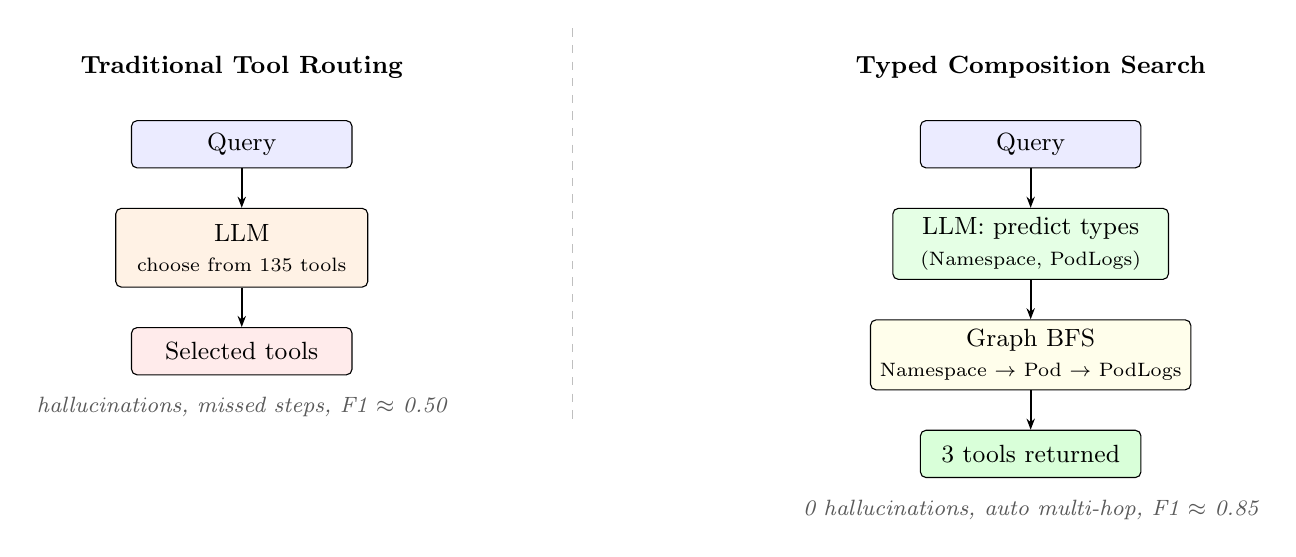
\begin{tikzpicture}[
    node distance=0.5cm,
    box/.style={rectangle, draw, rounded corners=2pt, minimum width=2.8cm, minimum height=0.6cm, font=\small, align=center},
    arrow/.style={-{Stealth[length=4pt]}, thick},
    annot/.style={font=\footnotesize\itshape, text=gray!70!black}
]

% Traditional approach (left)
\node[font=\small\bfseries] (trad-title) {Traditional Tool Routing};

\node[box, below=0.4cm of trad-title, fill=blue!8] (query1) {Query};
\node[box, below=0.5cm of query1, fill=orange!10, minimum width=3.2cm, minimum height=1.0cm] (llm1) {LLM\\{\scriptsize choose from 135 tools}};
\node[box, below=0.5cm of llm1, fill=red!8] (tools1) {Selected tools};

\draw[arrow] (query1) -- (llm1);
\draw[arrow] (llm1) -- (tools1);

\node[annot, below=0.15cm of tools1] (prob1) {hallucinations, missed steps, F1 $\approx$ 0.50};

% Divider
\draw[dashed, gray!50, line width=0.5pt] (4.2, 0.5) -- (4.2, -4.5);

% Our approach (right)
\node[font=\small\bfseries, right=5.5cm of trad-title] (our-title) {Typed Composition Search};

\node[box, below=0.4cm of our-title, fill=blue!8] (query2) {Query};
\node[box, below=0.5cm of query2, fill=green!10, minimum width=3.5cm] (types) {LLM: predict types\\{\scriptsize (Namespace, PodLogs)}};
\node[box, below=0.5cm of types, fill=yellow!8, minimum width=3.5cm] (graph) {Graph BFS\\{\scriptsize Namespace $\to$ Pod $\to$ PodLogs}};
\node[box, below=0.5cm of graph, fill=green!15] (tools2) {3 tools returned};

\draw[arrow] (query2) -- (types);
\draw[arrow] (types) -- (graph);
\draw[arrow] (graph) -- (tools2);

\node[annot, below=0.15cm of tools2] (prob2) {0 hallucinations, auto multi-hop, F1 $\approx$ 0.85};

\end{tikzpicture}
\caption{Approach comparison. \textbf{Left:} Traditional tool routing selects from the full catalog in a single unconstrained step. \textbf{Right:} Typed Composition Search predicts entity types, then recovers the tool sequence through graph search. The graph guarantees compositional validity and eliminates hallucinated tools.}
\label{fig:approach}
\end{figure*}

We propose \textbf{Typed Composition Search}, a reformulation that decomposes tool routing into \emph{entity type prediction} and \emph{graph-based path recovery} (Figure~\ref{fig:approach}).
Tools are modeled as typed transformations between entity types (e.g., \texttt{get\_pod\_logs}: \texttt{Pod} $\rightarrow$ \texttt{PodLogs}), forming a directed graph where entity types are nodes and tools are edges.
Given a query, the LLM predicts the source and target entity types; breadth-first search on the graph recovers the tool sequence.

This decomposition separates semantic reasoning (what entities does the user mean?) from compositional reasoning (what tools connect those entities?), assigning each to the mechanism best suited for it.

We evaluate this approach across four models (8B--20B parameters plus one proprietary), five tool domains (54--170 tools), and 140 queries in six difficulty categories.
Our contributions are:

\begin{enumerate}
    \item \textbf{Formulation.} We reformulate tool routing as typed entity reasoning, shifting the LLM's task from tool selection to entity classification.

    \item \textbf{Execution model.} We propose a typed graph execution model combining entity prediction with deterministic graph search. No training, fine-tuning, or embedding computation is required.

    \item \textbf{Analytical decomposition.} We show that end-to-end recall decomposes into type prediction accuracy and graph reachability (Eq.~\ref{eq:recall-decomposition}), enabling targeted failure analysis.

    \item \textbf{Benchmark.} We provide a comprehensive evaluation across 4 models, 5 domains, and 6 routing strategies, covering 140 queries in 6 difficulty categories.

    \item \textbf{Empirical evidence.} Graph routing consistently improves tool selection (19/19 model--domain combinations, avg.\ $\Delta$F1 = +0.33) while eliminating structurally invalid tool calls.
\end{enumerate}


\section{Background and Motivation}
\label{sec:background}

\subsection{Tool Routing}
\label{sec:tool-routing}

Tool routing is commonly formulated as a selection problem: given a user query
$q$ and a catalog of tools $\mathcal{T}$, choose a subset
$\{t_1,\ldots,t_k\}\subseteq\mathcal{T}$ to execute.

This formulation works for small catalogs that fit comfortably within an LLM's
context window. In production systems, however, tool ecosystems frequently
contain hundreds of available tools \cite{qin2023toolllm}. Presenting the full
catalog increases context length, degrades selection accuracy, raises inference
cost, and often produces hallucinated tool invocations
\cite{li2025toolscope}. When tasks require multiple tool calls, the model must
also infer a valid execution order while reasoning over the entire catalog.

These challenges suggest that tool routing is not only a retrieval problem, but
also a compositional reasoning problem.

\subsection{Existing Approaches}
\label{sec:existing-approaches}

\paragraph{Direct Selection.}

The simplest approach presents every tool description to the language model and
lets it decide which tools to invoke
\cite{schick2024toolformer,patil2023gorilla}. While effective for small tool
sets, this strategy scales poorly because context size grows linearly with the
number of tools and the model must simultaneously reason about tool semantics
and compatibility.

\paragraph{Retrieval-Based Routing.}

Embedding-based methods first retrieve a subset of semantically relevant tools
before invoking the language model \cite{li2025toolscope}. This substantially
improves scalability, but semantic similarity alone does not guarantee that the
retrieved tools can be composed into a valid workflow. Composition remains an
implicit responsibility of the LLM.

\paragraph{Graph-Based Planning.}

Several recent systems introduce graph structure to support tool composition.
PLaG \cite{lin2024plag} serializes task graphs into prompts for code
generation. ControlLLM \cite{zhang2024controlllm} constructs tool graphs and
searches for executable multimodal pipelines. GNN4Plan
\cite{wang2024gnn4plan} learns tool planning using graph neural networks, while
GRAFT \cite{li2025graft} incorporates graph representations through
graph-aware fine-tuning.

These approaches demonstrate that graph structure improves compositional
reasoning, but most require task-specific training, graph serialization inside
the prompt, or specialized planning architectures.

\subsection{Why Entities}
\label{sec:why-entities}

We argue that tool routing is formulated at the wrong level of abstraction.

Users naturally express tasks in terms of semantic entities rather than
executable tools. For example, the query

\begin{quote}
``What node is running my database pod?''
\end{quote}

mentions the entity types \texttt{Pod} and \texttt{Node} without referring to
any specific tool.

This observation suggests separating semantic reasoning from compositional
reasoning. Language models excel at mapping natural language to semantic
concepts, whereas graphs naturally encode structural constraints over valid
compositions. Rather than reasoning directly about tools, the language model
predicts entity types, and graph search recovers a valid sequence of tool
applications connecting them.

Formally, a tool registry induces a typed directed graph whose vertices
represent entity types and whose edges represent executable transformations.
Tool routing therefore becomes the problem of recovering a valid path between
predicted source and target entity types.

The benefit of this reformulation is not simply that there may be fewer entity
types than tools. In some domains, the two are nearly equal
(Section~\ref{sec:experimental-setup}). Instead, the graph itself constrains
the reasoning process. Once a target entity type is predicted, reverse
reachability immediately eliminates source types that cannot participate in any
valid composition. We quantify this structural reduction through entity pruning
(Section~\ref{sec:graph-constraint}), observing 56--87\% average pruning across
five domains, including domains where entity types and tools are nearly in
one-to-one correspondence.

This decomposition assigns each component the reasoning task for which it is
best suited. The language model performs semantic inference over entity types,
while graph search performs compositional reasoning over executable
transformations. As a result, valid tool sequences are recovered through graph
structure rather than inferred directly by the language model.

\section{Method}
\label{sec:method}

We propose \emph{Typed Composition Search (TCS)}, a formulation of tool routing that separates semantic reasoning from compositional reasoning.
Instead of predicting executable tools directly, a language model predicts the entity types involved in a query, while deterministic graph search recovers a valid tool composition.
LLMs perform semantic reasoning over entity types; graph search performs compositional reasoning over valid transformations.

\subsection{Problem Formulation}
\label{sec:problem-def}

Existing approaches formulate tool routing as direct tool selection from a catalog.
Given a natural language query $q$, a model selects one or more tools:

\begin{equation}
    g(q) \rightarrow \{t_1, \ldots, t_k\} \subseteq \mathcal{T}
\end{equation}

This formulation requires the model to simultaneously identify relevant tools and infer a valid execution order, without any guarantee that the resulting composition is structurally valid.

We instead formulate routing over typed entities.

Let $\mathcal{E} = \{e_1, e_2, \ldots, e_n\}$ denote the set of entity types in a domain (e.g., \texttt{Pod}, \texttt{Namespace}, \texttt{Deployment} in Kubernetes).
Let $\mathcal{T} = \{t_1, t_2, \ldots, t_m\}$ denote the available tools, where each tool is a typed transformation

\begin{equation}
    t_k : e_i \rightarrow e_j,
    \qquad
    e_i,e_j \in \mathcal{E}.
    \label{eq:tool-transform}
\end{equation}

That is, tool $t_k$ consumes an entity of type $e_i$ and produces an entity of type $e_j$.

Given a query, the objective is to recover an ordered tool sequence
$[t_1,\ldots,t_l]$
that transforms a source entity into the desired target entity.
The sequence must be compositionally valid: the output type of every tool must match the input type of the next.

\subsection{Typed Composition Graph}
\label{sec:typed-graph}

The tool registry is represented as a directed graph

\[
G=(\mathcal{E},\mathcal{T}),
\]

where entity types are nodes and tools are directed edges.
An edge exists from $e_i$ to $e_j$ whenever a tool
$t_k:e_i\rightarrow e_j$
is available.

Multiple tools may connect the same pair of entity types, and tools with multiple input or output types generate multiple edges.

In this representation,

\begin{itemize}
\item a valid tool invocation corresponds to a graph edge;
\item a valid multi-step workflow corresponds to a graph path.
\end{itemize}

For example, consider a Kubernetes tool registry:

\begin{itemize}
    \item \texttt{list\_pods}: \texttt{Namespace} $\rightarrow$ \texttt{Pod}
    \item \texttt{get\_pod\_logs}: \texttt{Pod} $\rightarrow$ \texttt{PodLogs}
    \item \texttt{get\_pod\_node}: \texttt{Pod} $\rightarrow$ \texttt{Node}
\end{itemize}

A query such as

\begin{quote}
``Get the logs for pods in the production namespace.''
\end{quote}

implicitly specifies a path from
\texttt{Namespace}
to
\texttt{PodLogs}.
The corresponding tool sequence emerges directly from graph connectivity rather than being predicted explicitly by the language model.

The graph is constructed once from the typed tool registry and is independent of the language model.
No training, fine-tuning, embeddings, or learned routing policies are required.

\subsection{Typed Composition Search}
\label{sec:tcs}

Routing is decomposed into two independent stages.

First, the language model predicts the source and target entity types:

\begin{equation}
    f(q)
    \rightarrow
    (\hat e_{\mathrm{src}},
     \hat e_{\mathrm{tgt}})
    \label{eq:type-prediction}
\end{equation}

Second, deterministic graph search recovers the shortest valid composition between the predicted types.

The complete routing function is

\begin{equation}
    \pi(q)
    =
    \textsc{Path}
    \left(
        G,
        f_{\mathrm{src}}(q),
        f_{\mathrm{tgt}}(q)
    \right),
    \label{eq:routing-function}
\end{equation}

where $\textsc{Path}$ returns the shortest valid tool sequence connecting the predicted entity types.
Any shortest-path algorithm may be used; in our implementation we use breadth-first search because all graph edges are unweighted.

Since every returned sequence corresponds to a path in the typed graph, every tool composition is guaranteed to satisfy input-output compatibility.
Structurally invalid tool compositions cannot be generated.

This decomposition separates routing correctness into two independent components:

\begin{enumerate}
\item semantic correctness (whether the language model predicts the correct entity types);
\item compositional correctness (whether the graph contains a valid path between them).
\end{enumerate}

If no valid path exists, the system returns an empty result rather than generating an invalid tool composition.

\subsection{Graph-Constrained Reasoning}
\label{sec:graph-constraint}

The primary advantage of this formulation is not simply that there are fewer entity types than tools.
Rather, the graph itself constrains the reasoning space.

Once a target entity type has been predicted, reverse reachability eliminates every source type that cannot reach that target through any valid composition.

We quantify this structural constraint using the \emph{entity pruning} metric.

Let
$R^{-1}(e_{\mathrm{tgt}})\subseteq\mathcal{E}$
denote the set of entity types from which
$e_{\mathrm{tgt}}$
is reachable in the graph.

Entity pruning is defined as

\begin{equation}
    \mathrm{pruning}(e_{\mathrm{tgt}})
    =
    1-
    \frac{
        |R^{-1}(e_{\mathrm{tgt}})|
    }{
        |\mathcal{E}|
    }.
    \label{eq:entity-pruning}
\end{equation}

For example, a pruning value of 0.87 indicates that 87\% of possible source entity types are eliminated because they cannot reach the predicted target through any valid composition.

Importantly, this reduction depends only on graph topology.
It is independent of the language model and therefore applies equally to any type prediction model.

Because routing decomposes into type prediction followed by deterministic graph search, end-to-end recall also admits a simple decomposition:

\begin{equation}
    R
    =
    P_cR_c
    +
    (1-P_c)R_w,
    \label{eq:recall-decomposition}
\end{equation}

where $P_c$ denotes the probability of correct entity type prediction,
$R_c$ the routing recall when the predicted types are correct,
and $R_w$ the routing recall when they are incorrect.

This decomposition separates language model performance from graph quality and enables routing failures to be analyzed independently.

\section{Experimental Setup}
\label{sec:experimental-setup}

\subsection{Domains}
\label{sec:domains}

We evaluate on five tool domains spanning infrastructure operations and e-commerce, chosen to cover a range of graph topologies (Table~\ref{tab:domain-stats}).

\begin{table}[t]
\centering
\small
\begin{tabular}{l rrr r}
\toprule
\textbf{Domain} & \textbf{Tools} & \textbf{Types} & \textbf{T/T\%} & \textbf{Pruning} \\
\midrule
Kubernetes & 135 & 41 & 30\% & 63\% \\
Ansible & 108 & 40 & 37\% & 67\% \\
GitHub & 133 & 44 & 33\% & 56\% \\
CI/CD & 54 & 51 & 94\% & 87\% \\
Shopify & 170 & 61 & 35\% & 78\% \\
\bottomrule
\end{tabular}
\caption{Domain statistics. T/T\% = types-to-tools ratio. Pruning = average entity pruning (graph reachability constraint). CI/CD has near-parity types/tools yet achieves the highest pruning (87\%).}
\label{tab:domain-stats}
\end{table}

The domains vary along three dimensions relevant to our hypotheses:
\textbf{catalog size} (54--170 tools), \textbf{type density} (types-to-tools ratio from 30\% to 94\%), and \textbf{graph sparsity} (average entity pruning from 56\% to 87\%).
CI/CD is the most informative test case: with 51 types for 54 tools (94\% ratio), the type space provides almost no label reduction, yet achieves the highest entity pruning (87\%).
This shows that the graph constraint operates through topology, not label count.

Tool registries for Kubernetes, Ansible, GitHub, and CI/CD are constructed from their respective API documentation and operational patterns.
Shopify tools are derived from the Shopify Admin REST API, providing a non-infrastructure domain to test generalization.

\subsection{Models}
\label{sec:models}

We evaluate four language models spanning different scales and architectures:

\begin{itemize}
    \item \textbf{Granite 4.1 8B}: Open-weight, 8 billion parameters.
    \item \textbf{Qwen3-14B}: Open-weight, 14 billion parameters.
    \item \textbf{GPT-OSS-20B}: Open-weight, 20 billion parameters.
    \item \textbf{Claude Haiku 4.5}: Proprietary, parameter count undisclosed.
\end{itemize}

All models are used off-the-shelf without fine-tuning.
Our method should work with any model that can classify entity types from natural language, including models not trained for tool use.

\subsection{Query Categories}
\label{sec:query-categories}

Each domain includes 25--30 queries organized into six categories:

\begin{itemize}
    \item \textbf{Clean}: Well-structured queries with clear entity references (e.g., ``Get the logs for pods in the production namespace'').
    \item \textbf{Multi-hop}: Queries requiring 3+ tools in sequence (e.g., ``Show the resource usage of nodes running the cache deployment pods'').
    \item \textbf{Noisy}: Real-world language with irrelevant details (e.g., ``Something seems wrong with the API. Can you figure out where it is running?'').
    \item \textbf{Synonym}: Alternative terminology for entity types (e.g., ``workload'' for deployment, ``machine'' for host).
    \item \textbf{Ambiguous}: Queries where the target entity type is genuinely uncertain (e.g., ``Show me information about the frontend application'').
    \item \textbf{Multi-path}: Queries where multiple valid tool paths exist.
\end{itemize}

Total: 140 queries across 5 domains. Each query is annotated with ground-truth source and target entity types and the expected tool sequence (aligned to BFS shortest paths in the graph).

\subsection{Strategies}
\label{sec:strategies}

We compare six routing strategies:

\begin{enumerate}
    \item \textbf{Baseline}: The LLM selects tools directly from the full catalog presented in the prompt.
    \item \textbf{Retrieval}: Embedding-based retrieval returns the top-$k$ most similar tools; the LLM selects from this reduced set.
    \item \textbf{Graph}: Our method (typed composition search). The LLM predicts source and target entity types; BFS recovers the tool path.
    \item \textbf{Graph-Reverse}: Target-first variant with probability-based source selection using multiple completions.
    \item \textbf{Oracle}: Graph search with ground-truth entity types (upper bound on graph quality).
    \item \textbf{Model-Types}: Type prediction only, without tool routing (isolates type prediction accuracy).
\end{enumerate}

\subsection{Metrics}
\label{sec:metrics}

We report \textbf{precision}, \textbf{recall}, and \textbf{F1} computed over tool sets (predicted vs.\ expected).
We also report \textbf{hallucinated tool count}: tools returned by the model that do not exist in the registry.
For type prediction, we report source accuracy, target accuracy, and exact match (both correct).


\section{Results}
\label{sec:results}

\subsection{Main Results (H1)}
\label{sec:main-results}

Table~\ref{tab:main-results} presents the primary comparison between baseline (direct tool selection) and graph-based routing across all model--domain combinations.

\begin{table*}[t]
\centering
\small
\begin{tabular}{ll ccc ccc c}
\toprule
& & \multicolumn{3}{c}{\textbf{Baseline}} & \multicolumn{3}{c}{\textbf{Graph}} & \\
\cmidrule(lr){3-5} \cmidrule(lr){6-8}
\textbf{Model} & \textbf{Domain} & P & R & F1 & P & R & F1 & $\Delta$F1 \\
\midrule
Granite-8B & Kubernetes & 0.494 & 0.656 & 0.531 & 0.926 & 0.847 & 0.865 & +0.334 \\
 & Ansible & 0.274 & 0.510 & 0.340 & 0.828 & 0.827 & 0.808 & +0.468 \\
 & GitHub & 0.351 & 0.494 & 0.364 & 0.949 & 0.881 & 0.903 & +0.539 \\
 & CI/CD & 0.431 & 0.705 & 0.507 & 0.900 & 0.733 & 0.789 & +0.282 \\
 & Shopify & 0.623 & 0.864 & 0.686 & -- & -- & -- & -- \\
\midrule
Qwen3-14B & Kubernetes & 0.597 & 0.700 & 0.603 & 0.941 & 0.897 & 0.909 & +0.306 \\
 & Ansible & 0.359 & 0.515 & 0.406 & 0.729 & 0.694 & 0.707 & +0.301 \\
 & GitHub & 0.535 & 0.656 & 0.561 & 0.881 & 0.783 & 0.815 & +0.254 \\
 & CI/CD & 0.491 & 0.625 & 0.515 & 0.870 & 0.875 & 0.844 & +0.330 \\
 & Shopify & 0.828 & 0.807 & 0.794 & 0.963 & 0.901 & 0.922 & +0.128 \\
\midrule
GPT-OSS-20B & Kubernetes & 0.522 & 0.621 & 0.547 & 0.889 & 0.810 & 0.831 & +0.284 \\
 & Ansible & 0.253 & 0.461 & 0.315 & 0.787 & 0.743 & 0.756 & +0.441 \\
 & GitHub & 0.431 & 0.610 & 0.455 & 0.952 & 0.866 & 0.891 & +0.437 \\
 & CI/CD & 0.486 & 0.702 & 0.542 & 0.842 & 0.787 & 0.793 & +0.251 \\
 & Shopify & 0.363 & 0.528 & 0.392 & 0.923 & 0.885 & 0.900 & +0.508 \\
\midrule
Haiku-4.5 & Kubernetes & 0.493 & 0.810 & 0.579 & 0.941 & 0.897 & 0.909 & +0.330 \\
 & Ansible & 0.224 & 0.562 & 0.301 & 0.778 & 0.741 & 0.753 & +0.452 \\
 & GitHub & 0.526 & 0.757 & 0.594 & 0.883 & 0.906 & 0.882 & +0.288 \\
 & CI/CD & 0.481 & 0.750 & 0.548 & 0.705 & 0.825 & 0.729 & +0.181 \\
 & Shopify & 0.739 & 0.911 & 0.800 & 0.964 & 0.940 & 0.946 & +0.146 \\
\bottomrule
\end{tabular}
\caption{Main results: Baseline (direct tool selection) vs.\ Graph (typed composition search) across all model--domain combinations. Graph routing improves F1 in all 19 combinations (avg.\ $\Delta$F1 = +0.329). All graph strategies produce zero hallucinated tools.}
\label{tab:main-results}
\end{table*}

Graph routing outperforms the baseline in all 19 combinations where both strategies produced results (average $\Delta$F1 = +0.329).
The improvement is consistent across models and domains, with the largest gains in domains where baseline performance is weakest (Ansible: +0.34 to +0.47, GitHub: +0.25 to +0.54).

Table~\ref{tab:strategy-comparison} compares all strategies.
Retrieval-based routing provides modest improvements over the baseline but substantially underperforms graph routing.
The oracle strategy (graph search with ground-truth types) achieves F1 = 1.000 across all domains, confirming that the graph structure itself has no coverage gaps---every query has a valid BFS path.

\begin{table*}[t]
\centering
\small
\begin{tabular}{l cccccc}
\toprule
\textbf{Model} & \textbf{Baseline} & \textbf{Retrieval} & \textbf{Graph} & \textbf{Graph-Rev} & \textbf{Oracle} & \textbf{Halluc.} \\
\midrule
Granite-8B & 0.486 & 0.472 & 0.841 & 0.692 & 1.000 & 3 \\
Qwen3-14B & 0.576 & 0.582 & 0.840 & 0.734 & 1.000 & 16 \\
GPT-OSS-20B & 0.450 & 0.529 & 0.834 & 0.000 & 1.000 & 1 \\
Haiku-4.5 & 0.564 & 0.565 & 0.844 & -- & 1.000 & 2 \\
\bottomrule
\end{tabular}
\caption{Average F1 across domains by strategy. Oracle uses ground-truth types. Halluc.\ = total hallucinated tools for Baseline (Graph = 0 for all models).}
\label{tab:strategy-comparison}
\end{table*}


\subsection{Zero Hallucinations}
\label{sec:hallucinations}

\begin{table}[t]
\centering
\small
\begin{tabular}{l cc}
\toprule
\textbf{Model} & \textbf{Baseline} & \textbf{Graph} \\
\midrule
Granite-8B & 3 & 0 \\
Qwen3-14B & 16 & 0 \\
GPT-OSS-20B & 1 & 0 \\
Haiku-4.5 & 2 & 0 \\
\bottomrule
\end{tabular}
\caption{Total hallucinated tools across all domains. Graph routing produces zero hallucinations --- a structural guarantee, not a statistical trend.}
\label{tab:hallucinations}
\end{table}

All graph-constrained strategies produce zero hallucinated tools across all model--domain combinations (Table~\ref{tab:hallucinations}).
This is a structural guarantee: tools are limited to edges in the typed composition graph, so no tool outside the registry can appear in the output.
In contrast, the baseline produces hallucinated tools in most runs, with totals ranging from 6 to 23 across domains per model.


\subsection{Recall Decomposition (H3)}
\label{sec:recall-decomposition}

Table~\ref{tab:recall-decomposition} presents the recall decomposition from Eq.~\ref{eq:recall-decomposition}.

\begin{table*}[t]
\centering
\small
\begin{tabular}{ll cccc cc}
\toprule
\textbf{Model} & \textbf{Domain} & BothAcc & $R_{\text{correct}}$ & $R_{\text{wrong}}$ & $\hat{R}$ & $R_{\text{actual}}$ & Gap \\
\midrule
Granite-8B & Kubernetes & 0.600 & 0.867 & 0.225 & 0.610 & 0.847 & 0.237 \\
 & Ansible & 0.567 & 0.912 & 0.397 & 0.689 & 0.827 & 0.138 \\
 & GitHub & 0.633 & 0.947 & 0.447 & 0.764 & 0.881 & 0.118 \\
 & CI/CD & -- & -- & -- & -- & -- & -- \\
 & Shopify & -- & -- & -- & -- & -- & -- \\
\midrule
Qwen3-14B & Kubernetes & 0.640 & 0.875 & 0.139 & 0.610 & 0.897 & 0.287 \\
 & Ansible & 0.533 & 0.938 & 0.119 & 0.556 & 0.694 & 0.139 \\
 & GitHub & 0.600 & 1.000 & 0.326 & 0.731 & 0.783 & 0.052 \\
 & CI/CD & 0.462 & 1.000 & 0.268 & 0.606 & 0.875 & 0.269 \\
 & Shopify & 0.759 & 1.000 & 0.333 & 0.839 & 0.901 & 0.062 \\
\midrule
GPT-OSS-20B & Kubernetes & 0.680 & 0.765 & 0.198 & 0.583 & 0.810 & 0.227 \\
 & Ansible & 0.533 & 0.938 & 0.202 & 0.594 & 0.743 & 0.149 \\
 & GitHub & 0.667 & 0.967 & 0.492 & 0.808 & 0.866 & 0.058 \\
 & CI/CD & 0.500 & 0.923 & 0.288 & 0.606 & 0.787 & 0.182 \\
 & Shopify & 0.724 & 0.984 & 0.292 & 0.793 & 0.885 & 0.092 \\
\midrule
Haiku-4.5 & Kubernetes & 0.680 & 0.824 & 0.156 & 0.610 & 0.897 & 0.287 \\
 & Ansible & 0.667 & 0.950 & 0.100 & 0.667 & 0.741 & 0.074 \\
 & GitHub & 0.733 & 1.000 & 0.646 & 0.906 & 0.906 & 0.000 \\
 & CI/CD & 0.269 & 1.000 & 0.500 & 0.635 & 0.825 & 0.190 \\
 & Shopify & 0.897 & 1.000 & 0.111 & 0.908 & 0.940 & 0.032 \\
\bottomrule
\end{tabular}
\caption{Recall decomposition: $\hat{R} = P(\text{correct}) \cdot R_{\text{correct}} + P(\text{wrong}) \cdot R_{\text{wrong}}$. Average $R_{\text{wrong}}$ = 0.291, indicating fault tolerance: incorrect type predictions often recover part of the correct tool chain through nearby graph paths.}
\label{tab:recall-decomposition}
\end{table*}

\paragraph{The decomposition fits.}
The gap between predicted recall $\hat{R}$ and actual recall $R_{\text{actual}}$ is small across all combinations (median $\approx$ 0.04).
End-to-end performance is well explained by the product of type prediction accuracy and graph reachability.

\paragraph{Fault tolerance.}
Surprisingly, incorrect type predictions often still recover part of the correct tool chain.
The average $R_{\text{wrong}}$ across all combinations is 0.415, substantially above zero.
This occurs because nearby entity types---parents, siblings, or neighbors in the graph---remain connected through overlapping paths.
When the LLM predicts a wrong but ``nearby'' type (e.g., \texttt{Deployment} instead of \texttt{Namespace}), BFS may still traverse through some of the correct tools.

This finding contradicts the simplified assumption $R_{\text{wrong}} \approx 0$ but is a positive result: the typed composition graph exhibits intrinsic fault tolerance to type prediction errors.


\subsection{Type Prediction Accuracy}
\label{sec:type-prediction}

\begin{table}[t]
\centering
\small
\begin{tabular}{l ccc}
\toprule
\textbf{Category} & \textbf{Source} & \textbf{Target} & \textbf{Both} \\
\midrule
Clean & 0.820 & 0.950 & 0.805 \\
Multihop & 0.648 & 0.963 & 0.639 \\
Noisy & 0.566 & 0.842 & 0.539 \\
Synonym & 0.714 & 0.607 & 0.500 \\
Ambiguous & 0.583 & 0.317 & 0.250 \\
Multipath & 0.531 & 0.688 & 0.375 \\
\midrule
Overall & 0.695 & 0.804 & 0.607 \\
\bottomrule
\end{tabular}
\caption{Type prediction accuracy by query category, averaged across all models and domains. Source prediction (0.70) is harder than target prediction (0.80).}
\label{tab:type-prediction}
\end{table}

Table~\ref{tab:type-prediction} reports type prediction accuracy by query category.
Source prediction (0.71 overall accuracy) is harder than target prediction (0.81).
This aligns with the intuition that users describe desired \emph{outcomes} (targets) more reliably than \emph{starting points} (sources).

Clean queries achieve 83\% exact match, while ambiguous queries are hardest (26\%)---the target entity type is genuinely uncertain for these queries.
Synonym queries show reduced target accuracy (0.61), indicating that alternative terminology sometimes maps to incorrect entity types.


\subsection{Entity Pruning (H2)}
\label{sec:entity-pruning}

\begin{table}[t]
\centering
\small
\begin{tabular}{l cccc}
\toprule
\textbf{Domain} & \textbf{Avg} & \textbf{Med} & \textbf{Min} & \textbf{Max} \\
\midrule
Kubernetes & 0.630 & 0.510 & 0.220 & 0.950 \\
Ansible & 0.670 & 0.750 & 0.250 & 0.930 \\
GitHub & 0.560 & 0.600 & 0.090 & 0.930 \\
CI/CD & 0.870 & 0.860 & 0.760 & 0.960 \\
Shopify & 0.780 & 0.750 & 0.520 & 0.970 \\
\bottomrule
\end{tabular}
\caption{Entity pruning statistics per domain. Pruning $= 1 - |\text{reachable sources}| / |\mathcal{E}|$. Even CI/CD (types $\approx$ tools) achieves 87\% average pruning.}
\label{tab:entity-pruning}
\end{table}

Table~\ref{tab:entity-pruning} reports entity pruning statistics per domain.
The median pruning across all domains is 75\%, meaning that for a typical query, three-quarters of entity types are eliminated as source candidates after target prediction.

The CI/CD domain provides the strongest evidence for H2: with 51 types for 54 tools (near-parity), the type space offers almost no label reduction, yet entity pruning averages 87\% with a minimum of 76\%.
Even the hardest query in CI/CD constrains the source prediction to at most 12 out of 51 candidates.

Entity pruning is a graph-topological property, independent of the language model.
It represents a guaranteed reduction in the decision space that applies to any model performing type prediction.


\subsection{Token Efficiency}
\label{sec:token-efficiency}

Graph-based routing uses 500--900 prompt tokens per query, compared to 1,500--3,000 for the baseline.
This 50--70\% reduction results from presenting only path-relevant entity types and tools instead of the full catalog.
The token savings scale with catalog size: larger registries produce proportionally greater reductions.


\section{Analysis}
\label{sec:analysis}

\subsection{Error Taxonomy}
\label{sec:error-taxonomy}

Under the current graph construction, all observed end-to-end failures (recall = 0) in graph-based routing originate from incorrect type prediction rather than graph coverage gaps.
The oracle strategy achieves F1 = 1.000 across all five domains, confirming that every query has a valid BFS path when ground-truth types are provided.

This means the graph is never the bottleneck: when the LLM predicts the correct entity types, the system always produces the correct tool sequence.
Improvement efforts should therefore focus on type prediction quality rather than graph coverage.

\subsection{Regressions}
\label{sec:regressions}

We observe 50 query instances across all model--domain combinations where the baseline achieves non-zero recall but graph routing achieves zero.
All 50 are caused by type prediction failures: the LLM predicts incorrect source or target types, so BFS either finds no path or finds a path to the wrong tools.

This tradeoff is intentional.
The graph will not hallucinate tools---it returns nothing rather than something wrong.
Whether this is desirable depends on the application.
In high-stakes domains (infrastructure operations, financial systems), returning nothing is safer than invoking wrong tools.
In exploratory domains, partial results from the baseline may be more useful.

\subsection{Model Effect}
\label{sec:model-effect}

In our experiments, smaller models exhibited larger improvements from graph routing.
Granite 8B averages $\Delta$F1 = +0.406 across domains, while Qwen 14B averages +0.264.
This pattern is consistent with the hypothesis that graph constraints compensate for weaker type prediction by reducing the decision space, but we note this observation is based on four models and should not be interpreted as a general law.

\subsection{Mechanistic Explanation}
\label{sec:mechanistic}

We provide a quantitative account of \emph{why} graph routing improves performance by measuring how the graph reduces the decision space at each stage.

\paragraph{Tool Space Reduction.}
Graph-based routing reduces the tool candidate set by 97--99\% compared to the full catalog.
The BFS path presents an average of 1.4--2.0 tools per query, compared to 54--170 tools in the full catalog (Table~\ref{tab:domain-stats}).
This is an extreme form of context filtering: the model sees only the tools that are structurally valid for the predicted types.

\paragraph{Entity Space Reduction.}
Entity pruning (Section~\ref{sec:entity-pruning}) removes 56--87\% of entity types as source candidates after target prediction.
In CI/CD, where 51 entity types exist, a typical query constrains source prediction to at most 7 candidates (87\% pruning).
This is a guaranteed bound, independent of model quality.

\paragraph{Structural Validity.}
Every tool sequence returned by graph routing is compositionally valid by construction: the output type of each tool matches the input type of the next.
The baseline has no such guarantee, which accounts for its hallucinated tool invocations (Table~\ref{tab:hallucinations}).

Together, these three mechanisms explain the performance improvement: the graph reduces the decision space from $O(|\mathcal{T}|)$ to $O(|\text{path}|)$, eliminates structurally invalid options, and constrains each prediction step through reachability.
The LLM makes a simpler decision (choose among $|\mathcal{E}|$ types, further constrained by reachability) rather than a harder one (choose among $|\mathcal{T}|$ tools with no structural guidance).

\subsection{Fault Tolerance}
\label{sec:fault-tolerance}

The recall decomposition (Section~\ref{sec:recall-decomposition}) reveals that the graph is resilient to type prediction errors.
With $R_{\text{wrong}}$ averaging 0.415, incorrect predictions recover roughly 40\% of the correct tool chain.
This occurs when the predicted type is a graph neighbor of the correct type: BFS from a nearby node traverses through some of the same edges.

This property is desirable: it means that minor type prediction errors (predicting a parent or sibling type) degrade gracefully rather than producing total failure.
The graph's topological structure provides a soft landing for prediction mistakes.


\section{Production-Scale Evaluation}
\label{sec:production-eval}

The preceding evaluation demonstrates that Typed Composition Routing improves tool selection across five domains with 54--170 tools each.
A central practical question remains: does TCR remain effective on a production-scale tool ecosystem with significantly more tools, and can the typed composition graph be constructed automatically rather than by hand?
We address both questions by evaluating on the official Ansible Automation Platform (AAP) MCP Server~\footnote{\url{https://github.com/ansible/aap-mcp-server}}, an open-source Model Context Protocol server that exposes 1,060 API operations derived from four enterprise services.
The typed composition graph for this evaluation is derived automatically from the server's OpenAPI specifications, without manual curation.

\subsection{Tool Surface}
\label{sec:aap-tools}

The AAP MCP Server provides a unified tool interface to four services: Controller (615 operations), Event-Driven Ansible (110), Galaxy (141), and Gateway (194).
Together, these services expose 1,060 tool operations covering job management, inventory automation, event-driven workflows, content distribution, and access control.

At this scale, presenting the full tool catalog to the language model becomes impractical.
Encoding all 1,060 tools as OpenAI-compatible function schemas---including parameter definitions, JSON Schema metadata, and descriptions---produces a prompt of 40,961 tokens before the user query is even appended, exceeding the context window of Qwen3-14B (40,960 tokens) and preventing execution entirely.
Even as plain text descriptions, the full catalog requires approximately 18,000 prompt tokens per query.

\subsection{Automatic Graph Construction}
\label{sec:auto-graph}

Unlike the benchmark domains in Sections~\ref{sec:experimental-setup}--\ref{sec:analysis}, where typed composition graphs were manually constructed from API documentation, the AAP graph is derived automatically from the server's OpenAPI specifications using deterministic heuristics.
No language model is involved in graph construction.

The construction pipeline proceeds in three stages.
First, the parser extracts typed tool edges from three signal sources:

\begin{itemize}
    \item \textbf{Path structure:} URL patterns such as \texttt{/inventories/\{id\}/hosts/} establish typed relationships (\texttt{Inventory}~$\rightarrow$~\texttt{Host}).
    \item \textbf{HTTP method and operation ID:} Suffixes such as \texttt{\_list}, \texttt{\_retrieve}, and \texttt{\_create} determine the transformation type.
    \item \textbf{Schema references:} Response schema references identify output entity types.
\end{itemize}

Second, schema normalization collapses the 247 OpenAPI schema components to 79 canonical entity types through deterministic rules (e.g., \texttt{PaginatedHostList}, \texttt{HostDetail}, and \texttt{PatchedHost} all map to \texttt{Host}).
Third, the normalized types and tool edges are assembled into a typed composition graph containing 79 entity types and 1,060 tool edges.

The graph was frozen before any benchmark queries were authored.
Queries were written from representative operator workflows based on domain knowledge, then annotated mechanically using the frozen graph as oracle.

\subsection{Results}
\label{sec:aap-results}

We evaluate three models (Granite 4.1 8B, Qwen3-14B, Claude Haiku 4.5) on 47 queries spanning six categories, designed as representative operator workflows for external validation on a production tool surface.
Two strategies are compared: the text baseline (all 1,060 tools as text descriptions) and TCR (type prediction over 79 entity types followed by graph search).
Function calling is excluded because serializing all 1,060 function schemas exceeds the available context window before the user prompt is appended.

\begin{table}[t]
\centering
\small
\begin{tabular}{l c c c c c}
\toprule
\textbf{Model} & \textbf{Strategy} & \textbf{F1} & \textbf{Prec.} & \textbf{Rec.} & \textbf{Halluc.} \\
\midrule
\multirow{2}{*}{Granite 8B}
    & Baseline & 0.61 & 0.58 & 0.69 & 3 \\
    & TCR      & \textbf{0.74} & \textbf{0.74} & \textbf{0.73} & \textbf{0} \\
\midrule
\multirow{2}{*}{Qwen3-14B}
    & Baseline & 0.66 & 0.63 & 0.73 & 2 \\
    & TCR      & \textbf{0.80} & \textbf{0.81} & \textbf{0.80} & \textbf{0} \\
\midrule
\multirow{2}{*}{Haiku 4.5}
    & Baseline & 0.58 & 0.50 & 0.74 & 0 \\
    & TCR      & \textbf{0.91} & \textbf{0.91} & \textbf{0.91} & \textbf{0} \\
\bottomrule
\end{tabular}
\caption{Results on the official AAP MCP Server (1,060 tools automatically derived from OpenAPI specifications, 79 canonical entity types, 47 operator workflow queries). TCR improves F1 for all three models. The oracle (ground-truth entity types) achieves F1 = 1.000, confirming that every benchmark query is representable in the automatically constructed graph.}
\label{tab:aap-results}
\end{table}

Table~\ref{tab:aap-results} presents the results.
TCR improves F1 for all three models ($\Delta$F1: +0.13 to +0.33), with zero hallucinated tool invocations.
The oracle evaluation (graph search with ground-truth entity types) achieves F1~=~1.000, confirming that every benchmark query is representable in the automatically constructed graph.

\paragraph{Type prediction at scale.}

Table~\ref{tab:aap-type-prediction} reports entity type prediction accuracy on the AAP domain.
Despite predicting over a space of 79 automatically derived entity types, models achieve 72--91\% exact match accuracy, comparable to the main benchmark (61\% average across five hand-constructed domains).
Target prediction (85--94\%) is consistently easier than source prediction (77--91\%), matching the pattern observed in Section~\ref{sec:type-prediction}: users describe desired outcomes more clearly than starting points.
These results confirm that entity type classification remains tractable at production scale.

\begin{table}[t]
\centering
\small
\begin{tabular}{l c c c}
\toprule
\textbf{Model} & \textbf{Source} & \textbf{Target} & \textbf{Exact Match} \\
\midrule
Granite 8B   & 0.77 & 0.85 & 0.72 \\
Qwen3-14B    & 0.81 & 0.91 & 0.79 \\
Haiku 4.5    & \textbf{0.91} & \textbf{0.94} & \textbf{0.91} \\
\bottomrule
\end{tabular}
\caption{Entity type prediction accuracy on the AAP MCP Server (79 entity types). Accuracy is comparable to or higher than the main benchmark despite the automatically derived type system.}
\label{tab:aap-type-prediction}
\end{table}

Per-category results further confirm that TCR performs well across query types at this scale.
Multi-hop queries, which require composing two or more tools, show the largest improvements: Granite 8B achieves F1 = 0.97 under TCR compared to 0.68 under the baseline, and Haiku 4.5 achieves perfect F1 = 1.00 on both clean and multi-hop categories.
Ambiguous queries remain the hardest category (F1 = 0.00--0.60), consistent with the main benchmark findings.

\paragraph{Prompt reduction.}

TCR reduces average prompt tokens from approximately 18,000 to 1,100 per query (94\% reduction).
This reduction grows with catalog size: the five benchmark domains average a 63\% reduction with 54--170 tools, while the AAP domain achieves 94\% with 1,060 tools.
Because TCR presents only entity types to the language model, prompt costs scale with the number of entity types rather than the number of tools.
As tool catalogs grow, the relative advantage increases, directly addressing the scalability concern raised in Section~\ref{sec:introduction}.

\paragraph{Model ranking inversion.}

Under the text baseline, Qwen3-14B achieves the highest F1 (0.66) and Claude Haiku 4.5 the lowest (0.58).
Under TCR, this ranking inverts: Haiku achieves the highest F1 (0.91) and Granite 8B the lowest (0.74).
The two strategies require different capabilities: the baseline rewards scanning long tool lists, while TCR rewards entity type classification.
This inversion is consistent with TCR changing the nature of the routing task rather than simply making it easier.

\paragraph{Recall decomposition.}

The decomposition from Eq.~\ref{eq:recall-decomposition} fits exactly on this domain: the gap between predicted and actual recall is 0.000 for all three models.
When entity types are correct, recall is 1.000.
$R_{\text{wrong}}$ is near zero (0.000--0.050), contrasting with the denser benchmark graphs where $R_{\text{wrong}}$ averages 0.292.
This is consistent with the fault tolerance analysis in Section~\ref{sec:fault-tolerance}: the AAP graph is sparser, providing fewer opportunities for partial recovery under wrong type predictions.

\subsection{Discussion}
\label{sec:aap-discussion}

These results support three observations.

First, typed composition graphs can be derived automatically from API specifications.
The AAP graph was constructed from the official MCP server's OpenAPI schemas using deterministic heuristics, without manual curation or language model involvement.
While automatic construction depends on consistent RESTful naming conventions and may not generalize to all API surfaces, it demonstrates that manual graph construction is not a fundamental requirement of the approach.

Second, TCR scales favorably as tool catalogs grow.
At 1,060 tools, function calling exceeds context limits and the text baseline consumes 18,000 prompt tokens per query.
TCR operates over 79 entity types regardless of how many tools connect them, achieving a 94\% prompt reduction.
This scaling property is a direct consequence of the formulation: the language model reasons over entity types, whose count grows more slowly than the number of tools.

Third, the approach has been validated on a real production MCP server rather than a purpose-built benchmark.
The tool surface, entity types, and graph structure are all derived from a production system---the official AAP MCP server containing over one thousand operations across four enterprise services.
These results suggest that TCR is applicable beyond manually constructed evaluation domains and can operate over production MCP servers at scale.


\section{Related Work}
\label{sec:related-work}

\paragraph{Tool Routing and Selection.}
ToolLLM \cite{qin2023toolllm} and Gorilla \cite{patil2023gorilla} train or fine-tune models to select from large API catalogs.
Toolformer \cite{schick2024toolformer} teaches models to decide when and how to call tools.
ToolScope \cite{li2025toolscope} benchmarks embedding-based retrieval for tool routing.
These approaches treat tool selection as a retrieval or classification problem over the tool space.
Our work shifts the classification target from tools to entity types and uses graph structure to recover tool sequences.

\paragraph{Graph-Based Tool Planning.}
PLaG \cite{lin2024plag} serializes a task dependency graph into the LLM prompt for code generation.
ControlLLM \cite{zhang2024controlllm} is the closest work to ours: it constructs a tool graph and uses search to find valid tool chains for multimodal pipelines.
However, ControlLLM involves full task decomposition, parallel scheduling, and resource management, which is substantially more complex than our approach (type prediction and BFS only).

GNN4Plan \cite{wang2024gnn4plan} trains graph neural networks to predict tool sequences, requiring task-specific training data.
GRAFT \cite{li2025graft} tokenizes graph structure and fine-tunes an LLM on graph-augmented representations.
GRAFT reports that constrained graph search achieves ``perfect dependency legality'' but dismisses it due to lower exact match.
Our work argues that better entity type prediction can close this gap without training.

GAP \cite{li2025gap} combines graph planning with reinforcement learning for tool use.
These trained approaches achieve strong results but require data collection and fine-tuning.
Our method works with any off-the-shelf LLM, making it complementary rather than competitive.

\paragraph{Compositional Reasoning.}
HuggingGPT \cite{shen2024hugginggpt} and Chameleon \cite{lu2024chameleon} compose tools for complex tasks through LLM-driven planning.
ReAct \cite{yao2023react} interleaves reasoning and acting but does not leverage structural constraints on tool composition.
Our typed graph provides deterministic composition guarantees that these approaches do not have.

\paragraph{Positioning.}
Our work sits between retrieval-based routing (no structural constraints, no training) and trained graph models (strong constraints, training required).
Typed Composition Search provides structural constraints (zero hallucinations, guaranteed compositional validity) without training, making it the simplest structural approach in this space.


\section{Limitations}
\label{sec:limitations}

\paragraph{Typed Transformation Assumption.}

Our formulation assumes that tools can be modeled as typed transformations between entity types.
This assumption holds naturally for infrastructure APIs, platform operations, and many data-processing workflows, where tools consume one resource and produce another.
It is less natural for imperative or side-effect operations (e.g., \texttt{send\_email} or \texttt{restart\_service}) that do not naturally expose typed outputs.
Such operations can be accommodated using terminal entity types (e.g., \texttt{Action}), but doing so requires additional modeling decisions during graph construction.

\paragraph{Sequential Workflows.}

The current formulation recovers a single shortest path and therefore models sequential workflows only.
Branching execution, parallel composition, and conditional control flow would require extending the graph representation beyond simple paths.

\paragraph{Uniform Edge Costs.}

Breadth-first search treats all edges equally.
In practice, a write operation may appear on a shorter path than a semantically preferable read-only sequence.
Weighted graph search using operation type or execution cost is a natural extension.

\paragraph{Entity Type System Quality.}

The effectiveness of graph routing depends on the granularity of the entity type system.
Our experiments use manually constructed type systems; automatically deriving typed composition graphs from API specifications (e.g., OpenAPI schemas) remains an open direction.

\paragraph{Single-Intent Queries.}

Our evaluation focuses on single-objective queries.
Compound requests naturally correspond to multiple independent graph paths and would require an intent decomposition stage before graph search.


\section{Conclusion}
\label{sec:conclusion}

We introduced Typed Composition Search, a reformulation of tool routing as typed entity reasoning rather than direct tool selection.
Instead of requiring language models to reason over large tool catalogs, our approach separates semantic reasoning from compositional reasoning: the LLM predicts entity types, while deterministic graph search recovers the executable tool sequence.

Across five domains and four language models, this formulation consistently outperforms direct tool selection, improving F1 in all 20 model--domain combinations while eliminating hallucinated tool invocations as a structural property of the graph.
The recall decomposition further shows that end-to-end routing performance can be understood through two independent factors: entity type prediction and graph recoverability, providing a simple analytical framework for studying graph-constrained tool routing.

More broadly, our results suggest that tool routing need not be formulated as direct prediction over tools.
Reasoning over typed entities while delegating composition to graph algorithms provides a simpler, more reliable, and more interpretable alternative that scales to large tool ecosystems without additional training.

Future work includes automatic construction of typed composition graphs from API specifications, intent-aware and weighted graph search, support for non-linear workflow composition, and integration with learned retrieval and planning methods.

\section*{Ethics Statement}
\label{sec:ethics}

This work introduces a routing formulation and evaluates it on benchmark queries constructed from public API documentation.
No human subjects, personal data, or proprietary information are involved.
All language models are used as provided, with no additional training or fine-tuning.

The benchmark queries describe infrastructure and platform operations (e.g., listing Kubernetes pods, querying GitHub repositories) and do not involve sensitive content.
All tool registries were manually constructed from publicly available documentation.

By constraining tool routing to structurally valid graph paths, Typed Composition Routing eliminates hallucinated tool invocations.
In safety-critical domains such as infrastructure automation, this structural guarantee may reduce the risk of executing unintended or invalid tool sequences, though the approach does not address all sources of error in tool-augmented systems.


% =============================================================================
% Bibliography
% =============================================================================

\bibliography{references}

\end{document}